% Owner: Shaurya. See docs/iml-planning/TEAM_WORK_SPLIT_V2.md section 8.
\section{Data and tasks}
\label{sec:data}

\paragraph{Dataset.} 298{,}445 anonymised parking-violation tickets issued by Bengaluru traffic
police across 54 stations over 151 days (10 Nov 2023 to 8 Apr 2024). Each record carries a
timestamp, station, H3 hexagon (resolutions 8 and 9), a severity weight, a peak-window weight,
and, held out of git, a device id identifying the issuing enforcement unit.

\paragraph{Task T1: station-day counts.} For each police station and day $d$, predict the ticket
count on $d$ from features built only from days strictly before $d$: counts 1, 7 and 14 days
back; 7- and 28-day rolling means; an expanding same-weekday mean; plus calendar features of $d$
itself (weekday, weekend, national holiday) and the station identity. Evaluated on 4
expanding-window folds with 14-day test blocks starting 2024-02-13, 2024-02-27, 2024-03-12 and
2024-03-26.

\paragraph{Task T2: hex-week hotspots.} For each H3 hexagon (resolution 8) and each of the 21
full calendar weeks in the data, predict whether that hexagon is a hotspot the \emph{following}
week: top 10\% of that week's hexagons by weekly impact
($\text{impact} = \sum \text{severity} \times \text{peak\_w}$ over the week's tickets). Features
use only weeks up to and including the current one: impact 1 to 4 weeks back, a 4-week rolling
mean, evening-ticket share, mean severity, junction share, and the mean impact of the hexagon's 6
ring-1 neighbours. Evaluated on 4 expanding-window folds over weeks [13,14], [15,16], [17,18] and
[19,20].

\paragraph{Is the evening gap real? (E1)} Figure~\ref{fig:evening-gap} plots ticket counts and
the number of distinct active enforcement devices by hour of day, each indexed to its own peak.
Both collapse together: 1{,}773 devices are active at 11:00 versus only 12 at 19:00, and the two
curves track each other closely, so the gap reflects enforcement presence actually dropping, not
an artifact of how tickets alone were counted.

On timestamp trustworthiness: every ticket's seconds field is fixed at 46 while minutes are
uniformly distributed (about 4{,}800 to 5{,}200 tickets per minute value), so the fixed seconds
are a data-entry or anonymisation artifact that does not affect hour- or day-level timing.
Device-level shift analysis (each device's first and last active hour per day) corroborates the
station-level pattern rather than being an aggregation artifact: the median device-day runs from
hour 6 to hour 8, squarely inside the 02:00--12:00 window where both series peak, collapsing to
near zero from 15:00 onward. Weekday and weekend shifts start and end within about 15 minutes of
each other on average, so the evening gap is a structural daily feature of enforcement, not a
day-of-week artifact.

\begin{figure}[t]
 \centering
 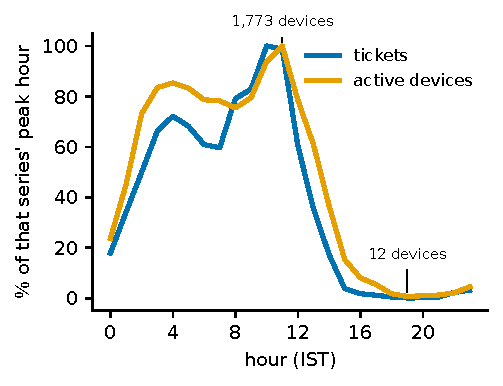
\includegraphics[width=\linewidth]{F1_evening_gap}
 \caption{Tickets and distinct active enforcement devices by hour (IST), each indexed to its own
 peak hour. Both collapse from the early afternoon onward and recover only slightly after
 22:00.}
 \label{fig:evening-gap}
\end{figure}

\paragraph{Do stations differ in when, not how much? (E6)} We build a 54$\times$24 matrix of each
station's hourly ticket share (rows sum to 1, so overall volume differences are removed by
construction) and run PCA. PC1 explains 30.3\% of variance and PC2 24.8\%
(\texttt{results/tables/E6\_unsup.csv}). As Figure~\ref{fig:pca} shows, PC1 loads negative across
00:00--09:00 and strongly positive across 10:00--14:00: a pure early-versus-late-morning timing
contrast, which confirms the hypothesis that stations separate by \emph{when} they record rather
than \emph{how much}. K-Means ($k=2..6$, chosen by silhouette) selects $k=2$ (silhouette 0.21,
weak but real separation): a 35-station ``pre-dawn'' archetype peaking at 04:00 and a 19-station
``late-morning'' archetype peaking at 11:00.

\begin{figure}[t]
 \centering
 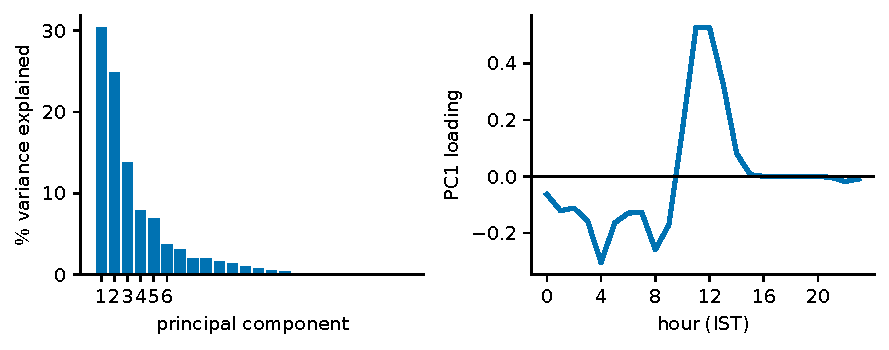
\includegraphics[width=\linewidth]{F4_pca_kmeans}
 \caption{Left: variance explained by each principal component of the station timing-profile
 matrix. Right: PC1's loading at each hour, showing the early-versus-late-morning timing
 contrast that separates the two K-Means archetypes.}
 \label{fig:pca}
\end{figure}
